
% \section{Methods of signal reconstruction}
\subsection{Photometry}
\label{sec:signal}

A dedicated KID readout system has been developed by \citet{2013A&A...551L..12C}
and successfully used for \nika\ and \nika2\ \todo{which paper should we cite
  here, all ?}. We here summarize its main characteristics and the observables
that are relevant for our simulation work. We then present two ways to use them
to derive the photometry.

%% To convert the $\I(t)$ and $\Q(t)$ that
%% describe the resonance frequency shift $\delta f_0$ to the absorbed optical
%% power $\delta P_{opt}$. We have devised two ways to relate these
%% quantities. Both rely on a specific electronic modulation readout devised by
%% \citet{2013A&A...551L..12C} that we summarize first.

\subsubsection{Modulated readout technique}

\begin{figure}
  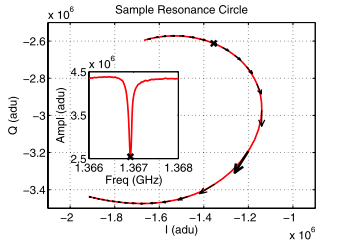
\includegraphics[clip,angle=0,width=\columnwidth]{Figures/resonance-circle.png}
  \caption{Trajectory of $\I$ and $\Q$ during a frequency sweep around the
    resonance of a KID. The arrows represent $(\di,
    \dq)$. \citep{2013A&A...551L..12C}}
  \label{circle-iq}
\end{figure}

The excitation tone frequency of a KID is modulated by a local oscillator with a
known frequency shift. This provides two values $f_{\pm} = f_0 \pm \delta
  f_{LO}/2$ with $\delta f_{LO} \simeq 1$\,kHz. The ``In-phase'' in
``in-Quadrature'' amplitudes $i(t)$ and $q(t)$ then read:

\begin{equation}
(i(t), q(t)) = (\frac{i(f_{+}) +
    i(f_{-})}{2},
\frac{q(f_{+}) + qf_{-})}{2}),
\end{equation}

and the differential values are :

\begin{equation}
\label{gradient}
(\di(t), \dq(t)) =
\left(\frac{i(f_{+}) - i(f_{-})}{\delta f_{LO}},
\frac{q(f_{+}) - q(f_{-})}{\delta f_{LO}}\right).
\end{equation}

These quantities are represented on Fig. \ref{circle-iq}. In this paper, we take
typical laboratory values and assume that $i$ and $q$ are sampled at
880\,Hz. This high acquisition rate is allowed by the sub-millisecond time
constant of the KIDs. For most experiments, such a high sampling rate is not
required and we average these measures over 40~samples to produce
four secondary quantities at 22\,Hz:

\begin{eqnarray}
\I  &=& \sum^{N_{m}=40}_{p=1} i_{p},\\
\Q  &=& \sum^{N_{m}=40}_{p=1} q_{p},\\
d\I &=& \sum^{N_{m}/2=20}_{p=1} i_{2p} - i_{2p-1},\\
d\Q &=& \sum^{N_{m}/2=20}_{p=1} q_{2p} - q_{2p-1}.
\end{eqnarray}

With these quantities in hand we have several ways to derive the transmitted
signal. They are presented in the following paragraph.

\subsubsection{\rf}
If a variation $\Delta\I(t)$, $\Delta\Q(t)$ is observed between successive ($\I$,
$\Q$) points, it is possible to estimate the shift of the resonant frequency
$\Delta f_{0}$ between these two samples by comparing ($\Delta \I$, $\Delta \Q$)
with the gradient $(\di,\dq)$ induced by the known $\delta
f_{0}$ of the local oscillator. This is done by a scalar projection of ($\Delta\I$,
$\Delta\Q$) on $(\di,\dq)$ that is tangent to the resonance circle. To have a
cleaner estimation of the latter, we take its running average over 50
points that we write $\langle . \rangle_{50}$ \citep{2014A&A...569A...9C}:

\begin{equation}
\label{eq:Rf}
\Delta f_{0} = \delta f_{LO} \frac{\Delta \I\, \langle \di
  \rangle_{50}
+ \Delta \Q\, \langle \dq \rangle_{50}}{\langle \di
  \rangle_{50}^{2}
 + \langle \dq \rangle_{50}^{2}},
\end{equation}

Note that this average is performed only on the tangent vector $(\di,\dq)$ so
that $\Delta f_0$ is sampled like $\I$ and $\Q$ at 22\,Hz. This method has been
successfully used in \todo{XXXX}, but can be affected by some systematic
uncertainty and be a source of non-linearity. Indeed, $(\di,\dq)$ is tangent to
the $(\I,\Q)$ circle for a fixed background optical power, while, in principle,
the incident optical power that induces the observable $(\Delta \I, \Delta \Q)$
should distort the resonance circle to some extent. As a consequence, the
observed $(\I,\Q)$ trajectory is not precisely parallel to the $(\di,\dq)$
direction. Early laboratory and on-site tests have shown that this approximaton
leads to a reconstruction of point source fluxes better than 2\%
\citep{2013A&A...551L..12C}. In this work, we improve this upper limit on
simulations and assess the impact of this error on futures CMB polarization
measurements.

\subsubsection{Circle fit : Cf}

\begin{figure}
\includegraphics[clip, angle=0, width=\columnwidth]{Figures/circle_zres.eps}
\caption{Bottom: location of $\I$ and $\Q$ when a KID observes a point source of
  various fluxes. Top: ratio of the distance between $(\I,\Q)$ and the center of
  the fitted circle over the radius of this circle. All the points on the pure
  imaginary line at $\I=1$ are the result of the transformation of the circle
  into $Z_{res}$ according to eqs.~(\ref{eq:z_res}) and
  (\ref{eq:scale_rotate}).}
\label{fig:circle_zres}
\end{figure}

\todo{ref to the circular nature of (I,Q): \cite{2011ApJS..194...24M}}.\\

To improve \rf, we developed a new technique that fully exploits the circular
nature of the $(\I,\Q)$ trajectory, hereafter called \cf. It is
  based on the transformation property of a circle in the complex plane into a
  straight line. Indeed, let us consider a circle centered on $(0,1/2)$ with a
  radius $1/2$ and compute its inverse:

\begin{eqnarray}
Z_{ref} &\equiv&\frac{1}{2} + \frac{1}{2}e^{i\phi}\,, \\
&=&\cos\frac{\phi}{2}e^{i\phi/2}\,,\\
Z_{res} &\equiv& 1/Z_{ref}\,, \label{eq:z_res} \\
&=&1-i\tan\frac{\phi}{2}\,.
\label{eq:z_res}
\end{eqnarray}

$Z_{res}$ is a straight line and along this line $Z$ varies linearly with
$\phi$ for small values of $\phi$. Experimentally, we are in this regime
when the signal is weak and when $\phi$ is defined w.r.t.~ the $(O,C)$ axis
as defined on Fig.~\ref{fig:circle_zres}. We thus fit the radius $r$ and the
center $(\I_c,\Q_c)$ of our measurement circle $Z=\I+j\Q$. Defining
$\alpha=\arctan\Q_c/\I_c$, we scale, rotate and translate this
circle to the $Z_{res}$ circle according to

\begin{equation}
Z_{ref} = \left(\begin{array}{c}
\I_{ref}\\
\Q_{ref}\end{array}\right) = 
\frac{-1}{2r}\left(\begin{array}{rr}
\cos\alpha & \sin\alpha\\
-\sin\alpha & \cos\alpha\end{array}\right)
\left(\begin{array}{c}
\I-\I_c\\
\Q-\Q_c\end{array}\right) +
\left(\begin{array}{c}
1/2\\
0\end{array}\right)
\label{eq:scale_rotate}
\end{equation}

The result of this transformation is shown on Fig.~\ref{fig:circle_zres}. A
variation of the signal $(\Delta\I,\Delta\Q)$ leads to a variation
$\Delta\phi$ along $Z$ that is proportional to the frequency shift $\Delta f$
that we are after to determine photometry. To derive the calibration between
these two quantities, we once again rely on the $(\di,\dq)$ that is induced by
the known $\delta f_{LO}$. Applying transformation (\ref{eq:scale_rotate}) to
$(\di,\dq)$, we obtain the corresponding variation $dy = Im(dZ_{res})$. The
final derivation of $\Delta f$ corresponding to $(\Delta\I,\Delta\Q)$ requires
the integration of $dy/\delta f_{LO}$. For the sake of simplicity, we fit
$Im(dZ_{res})$ as a polynomial of $dy/\delta f_{LO}$ that is therefore trivial
to integrate.

%% \begin{equation}
%% \tan\frac{\delta\phi}{2} \simeq \frac{\delta\phi}{2} +
%% \frac{(\delta\phi)^3}{15}
%% \end{equation}

{\color{blue} 
\subsection{Non linearity characterization with simulations}

\begin{figure}
\center
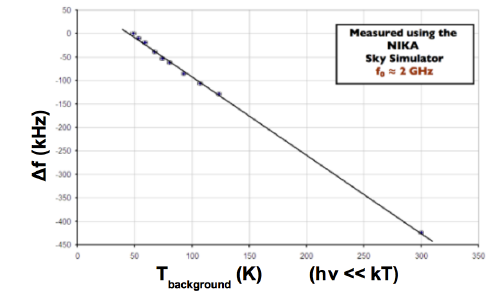
\includegraphics[clip, angle=0, width=\columnwidth]{Figures/KID-linearity-Monfardini2014.png}
\caption{KID linearity demonstrated in laboratory under realistic
  conditions. The plot shows the frequency shift of the resonance as a function
  of the optical background temperature (K). Solid line : linear fit of the
  experimental points. Credits : \citet{2014JLTP..176..787M}.}
\label{fig:KID-lin}
\end{figure}

Laboratory measurements with \todo{XXXX describe set up XXX} have shown that
KIDs are linear over a wide range of backgrounds
(Fig.~\ref{fig:KID-lin}). However, for these measurements, $\Delta f$ was not
reconstructed as described in the previous section, and we want to characterize
our formalism up to $\epsilon$ of the order of $10^{-5}-10^{-6}$. We simulate
the measure of point source by a KID and show how linear this measure remains in
various contexts. Non linearity could appear when the source is very bright
(such as planets of several tens of Jy) and the density of charge carriers is
altered. This leads to $(\I,\Q)$ meaures that leave the resonance circle, hence
invalidating the approximations made in the photometric equations of the
previous section. A second possible source of non linearity is the instrument
scanning speed. Indeed, even if the source is moderately bright, if it is
scanned too fast, $(\Delta\I,\Delta\Q)$ could be far from the tangent vector
$(\di,\dq)$ which would alter their linear relation. In this paragraph, we
explore both cases. We simulate the observation of a point source with a flux
that we vary between \todo{1 and 500\,Jy TBC}. We assume that our instrument has
a 11\,arcsec FWHM Gaussian beam like the polarized 1\,mm channel of \nikad. We
also vary the scanning speed of our virtual instrument while keeping a minimum
of 3~samples per FWHM to respect the Nyquist criterion.

Modulation of the polarization by a rotating Half Wave Plate (HWP) like in
\nika\ and \nikad\ creates a background modulation equivalent to several tens to
hundreds of Jy at frequencies close to the HWP rotation harmonics
\citep{2017A&A...599A..34R}. After early tests by \todo{cite Hildebrand in the
  80's or so ?}, this kind of modulating device has been left aside for
\todo{20~TBC} years in the context of millimetric observations. With the
improvement of technologies it progressively came back in the landscape, in
particular with pioneering experiments like \emph{Maxipol}
\citep{2007ApJ...665...42J} and \emph{EBEX} \citep{2010SPIE.7741E..1CR}. It is
now more and more common and is considered as the leading option for future
satellite designs such as \emph{LiteBIRD} \todo{add ref}. Such a background must
be accounted for in the simulations.






%% In the context of a CMB experiment mapping a large fraction of the sky, one
%% should also consider the CMB dipole with its 6.73\,mK peak to peak \todo{ADD
%%   REF} converts into a \todo{XXX\,Jy} signal \todo{Account for the bandpass
%%   !!}. It can displace the zero level $Z$ along the circle so that a
%% bright source would enter the non linear regime sooner than expected. This is
%% also true for strong Galactic emission like that of Dust at frequencies above
%% $\sim 100$\,GHz. It is even truer for the background modulation induced by a
%% rotating Half Wave Plate (HWP). After early tests by \todo{cite Hildebrand in
%%   the 80's or so ?}, this kind of modulating device has been left aside for
%% \todo{20~TBC} years in the context of millimetric observations. With the
%% improvement of technologies, it progressively came back in the landscape, in
%% particular with pioneering experiments like \emph{Maxipol}
%% \citep{2007ApJ...665...42J} and \emph{EBEX} \citep{2010SPIE.7741E..1CR}. It is
%% now more and more common and is considered as the leading option for future
%% satellite designs such as \emph{LiteBIRD} \todo{add ref.}. \nika\ has used a
%% fast and continously rotating HWP and saw strong parasitic signal synchronous
%% with the HWP rotation harmonics \citep{2017A&A...599A..34R} like \emph{Maxipol}
%% and \emph{EBEX} (cf.~Fig.~\ref{fig:hwp_power_spectrum}). The amplitude of this
%% signal is comparable to bright planets at several tens of Jy and could also bias
%% the average position of the $Z$ measurement and hence the photometry.

}







%%  The idea of this
%% method is to project $\I$, $\Q$, $d\I$, $d\Q$, onto an axis $y'$ which is
%% as linear as possible with frequency and thus with the incident optical
%% power. Let's denote $Z = \I + j\Q$, near the resonance circle we have:
%% 
%% \begin{equation}
%% f - f_{0}= \frac{w}{2} \tan \frac{\phi}{2}.
%% \label{eq:hyp-f}
%% \end{equation}
%% 
%% \todo{what are $w$ and $\phi$?}\\
%% The idea is to construct $y'$ from a circle $Z$. The inverse of $Z$ is a circle
%% but we can normalize it to transform it into an infinite radius circle that is
%% expected to be linear with the KID frequency.  To do so we define a reference
%% circle which is centered on ($\frac{1}{2},0$) and has a radius of $\frac{1}{2}$,
%% after using trigonometric relations we obtain :
%% 
%% \begin{equation}
%% Z_{ref} = \cos \frac{\phi}{2} e^{j \phi/2}.
%% \label{eq:Zref}
%% \end{equation}
%% 
%% If we inverse Eq.~(\ref{eq:Zref}), we have : 
%% \begin{equation}
%% Z_{res} = 1 - j \tan \frac{\phi}{2}.
%% \label{eq:Zres}
%% \end{equation}
%% 
%% The imaginary part of Eq.~(\ref{eq:Zres}) is linearly dependant on the frequency
%% defined in Eq.~(\ref{eq:hyp-f}), and represents the new axis $y'$.
%% 
%% From the KID model we have $Z=\I+j\Q$. We do a series of transformations on this
%% circle to make it identical to the reference circle, the final result is named
%% $Z'$, with $Z'=p[ZM_{r} + T]$. p is the scaling factor, T represents the
%% translation and $M_{r}$ is the rotation matrix :
%% 
%% \begin{equation}
%% M_{r} = 
%% \begin{pmatrix}
%% 	\cos \alpha & \sin \alpha \\
%% 	-\sin \alpha & \cos \alpha
%% \end{pmatrix} .
%% \end{equation}
%% 
%% 
%% First we rotate $Z$ :
%% \begin{equation}
%% Z' = 
%% \begin{pmatrix}
%% 	\cos \alpha & \sin \alpha \\
%% 	-\sin \alpha & \cos \alpha
%% \end{pmatrix}
%% \begin{pmatrix}
%% 	\I\\
%% 	\Q
%% \end{pmatrix}
%% =
%% \begin{pmatrix}
%% 	\I\cos \alpha + \Q\sin \alpha\\
%%   - \I\sin \alpha + \Q\cos \alpha
%% \end{pmatrix}.
%% \end{equation}
%% 
%% Then we translate and rescale it, to obtain $Z'=\I'+j\Q'$ with : 
%% \begin{eqnarray}
%% \I' &=& \frac{1}{2r}[(\I-x_{c}) \cos \alpha + (\Q - y_{c}) \sin \alpha] + \frac{1}{2}, \\
%% \Q' &=& \frac{1}{2r}[-(\I-x_{c}) \sin \alpha + (\Q - y_{c}) \cos \alpha]. \\
%% \end{eqnarray}
%% 
%% ($x_{c}, y_{c}$), r and $\alpha$ respectively, the center, radius and rotation
%% angle of the initial circle. The derivative of the inverse of $Z'$ is
%% $dZ_{res}=-dZ'/Z'^{2}$, with :
%% 
%% \begin{eqnarray}
%% dZ' &=& d\I' + jd\Q',\\
%% d\I' &=& -\frac{1}{2r}(d\I \cos \alpha + d\Q \sin \alpha), \\
%% d\Q' &=& \frac{1}{2r}(-d\I \sin \alpha + d\Q \cos \alpha).
%% \end{eqnarray}
%% 
%% The imaginary part of $Z_{res}$ and $dZ_{res}$ represent respectively $y'$ and
%% $dy'$ which are proportional to the KID frequency. We can use these quantities
%% to calibrate $y'$ and derive the frequency of the KID. In fact, according to the
%% hypothesis in Eq.~(\ref{eq:hyp-f}), $f$ is a polynomial, so to reconstruct the
%% shift of the resonant frequency we can fit $\frac{\Delta f}{dy_{3}} = R_{n}(y')$
%% by a polynomial function, where $R_{n}$ is a polynomial function with a degree
%% $n$. It is then easy to integrate $R_{n}$ into $P_{n+1}$, with
%% $\overset{.}{P_{n+1}}=R_{n}$ to obtain the relative frequency of the KID :
%% 
%% \begin{equation}
%% f - f_{0} = P_{n+1}(y')
%% \end{equation}
%% 
%% \todo{keep for global conclusion:} In conclusion, because we can not directly
%% measure the optical power from a KID, new methods were developed to monitor the
%% shift of the resononance frequency of the detector. First with the modulated
%% readout technique we can calculate four quantities : $\I$, $\Q$, $\di$,
%% $\dq$. With these quantities in hand, we can monitor the shift of the resonant
%% frequency and derive the corresponding incident power ny using the two methods
%% that were developed : \rf\ which is already successfully used in \nika\ and
%% \nika2\ (see \citep{2014A&A...569A...9C}) , and \cf\ which is an improvement
%% from \rf . In this paper, we compare these two methods in terms of linearity. To
%% do so, in the next sections we do simulations of observations by a KID and we
%% use \rf\ and \cf\ to reconstruct the signal. We then study the impact of the KID
%% non-linearity on the search for B modes polarization of the CMB.
